\documentclass[10pt]{article}
\usepackage[letterpaper,margin=0.58in]{geometry}
\usepackage{amsmath,amssymb,amsthm,mathtools}
\usepackage{microtype}
\usepackage{enumitem}
\usepackage{xcolor}
\usepackage{tikz}
\usetikzlibrary{arrows.meta,positioning,fit,calc}
\usepackage[hidelinks]{hyperref}

\definecolor{proved}{HTML}{287A4B}
\definecolor{finite}{HTML}{9B6A00}
\definecolor{open}{HTML}{B3261E}
\newtheorem{proposition}{Proposition}
\newtheorem{lemma}[proposition]{Lemma}
\newcommand{\F}{\mathbb F}
\newcommand{\E}{\mathcal E}
\newcommand{\proved}{\textcolor{proved}{\textbf{PROVED}}}
\newcommand{\finite}{\textcolor{finite}{\textbf{FINITE}}}
\newcommand{\openstatus}{\textcolor{open}{\textbf{OPEN}}}
\setlist{nosep,leftmargin=1.3em}
\setlength{\parindent}{0pt}
\setlength{\parskip}{2.5pt}
\setlength{\textfloatsep}{4pt}
\setlength{\abovedisplayskip}{4pt}
\setlength{\belowdisplayskip}{4pt}

\title{\vspace{-2.2em}Half-degree irreducibles over $\F_2$:\\a proof roadmap with one missing bridge}
\author{Michael Bommarito}
\date{21 August 2026}

\begin{document}
\maketitle
\vspace{-1.8em}
\begin{center}
\fcolorbox{open}{open!5}{\parbox{0.94\linewidth}{\centering
\textbf{Status.} This is not a proof of the Kaser--Lemire conjecture.
The red estimate in Figure~\ref{fig:roadmap} remains open; all subsequent
claims are conditional on it.}}
\end{center}
\vspace{-0.5em}

\begin{abstract}
Kaser and Lemire observed that Barrett reduction over $\F_2$ is especially
cheap when an irreducible polynomial $f$ of degree $n$ satisfies
$\deg(f-x^n)\leq\lfloor n/2\rfloor$, and conjectured existence for every
$n$. We give a compact audit of an attempted proof. Reciprocal polynomials,
logarithmic differentiation, and M\"obius inversion reduce the problem to a
signed ray-class trace. A characteristic-two inverse-energy theorem supplies
the wrapped bilinear input, and exact Haar and order decompositions eliminate
all coarse and low-order frequencies. What remains is one uniform high-Witt
signed-discrepancy estimate. We state it exactly and show how it would close
both parity endpoints. Computation independently verifies $n\leq400$ but is
not used as evidence for the missing estimate.
\end{abstract}

\section{The proof chain at a glance}

Put $\ell=\lceil n/2\rceil-1$. The following diagram distinguishes theorem
from experiment and conjectural bridge.

\begin{figure}[h]
\centering
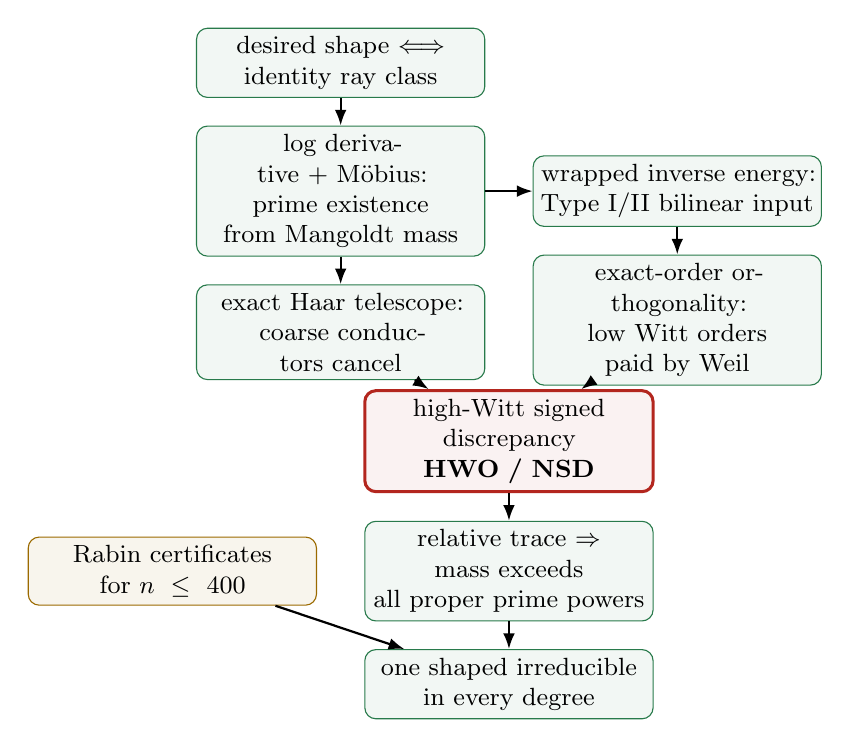
\begin{tikzpicture}[
  node distance=3.5mm and 6mm,
  box/.style={draw,rounded corners,align=center,text width=3.45cm,
              minimum height=8mm,inner sep=3pt,font=\small},
  p/.style={box,draw=proved,fill=proved!6},
  f/.style={box,draw=finite,fill=finite!7},
  o/.style={box,draw=open,fill=open!6,line width=1.1pt},
  arr/.style={-{Latex[length=2mm]},thick}
]
\node[p] (shape) {desired shape $\Longleftrightarrow$\\identity ray class};
\node[p,below=of shape] (mobius) {log derivative + M\"obius:\\prime existence from Mangoldt mass};
\node[p,below=of mobius] (haar) {exact Haar telescope:\\coarse conductors cancel};
\node[p,right=of mobius] (energy) {wrapped inverse energy:\\Type I/II bilinear input};
\node[p,below=of energy] (orders) {exact-order orthogonality:\\low Witt orders paid by Weil};
\node[o,below=8mm of $(haar)!0.5!(orders)$] (hwo) {high-Witt signed discrepancy\\\textbf{HWO / NSD}};
\node[p,below=of hwo] (close) {relative trace $\Rightarrow$ mass exceeds\\all proper prime powers};
\node[f,left=of close] (finite) {Rabin certificates\\for $n\leq400$};
\node[p,below=of close] (result) {one shaped irreducible\\in every degree};
\draw[arr] (shape)--(mobius);
\draw[arr] (mobius)--(haar);
\draw[arr] (mobius)--(energy);
\draw[arr] (energy)--(orders);
\draw[arr] (haar)--(hwo);
\draw[arr] (orders)--(hwo);
\draw[arr] (hwo)--(close);
\draw[arr] (close)--(result);
\draw[arr] (finite)--(result);
\end{tikzpicture}
\caption{The current dependency graph. Green is proved, gold is finite
verification, and red is the sole load-bearing open estimate.}
\label{fig:roadmap}
\end{figure}

\section{Proved reductions, step by step}

\textbf{1. Reciprocal ray class (\proved).}
For $j\geq0$ set
\[
 \E_j=(1+x\F_2[x])/(x^{j+1}),\qquad |\E_j|=2^j,
\]
and, for monic $F$, let
$\langle F\rangle_j=x^{\deg F}F(x^{-1})\pmod{x^{j+1}}$.
The bound $\deg(f-x^n)\leq\lfloor n/2\rfloor$ is exactly
$\langle f\rangle_\ell=1$. Thus the conjecture asks for a degree-$n$ prime
in one prescribed Hayes ray class.

\textbf{2. Mangoldt population and prime extraction (\proved).}
Define
\[
 N_j(b)=\sum_{\substack{F\text{ monic},\ \deg F=n\\
                 \langle F\rangle_j=b}}\Lambda(F).
\]
Exact logarithmic differentiation counts prime powers with weight $\Lambda$;
M\"obius inversion, or direct subtraction here, then extracts primes. At the
odd endpoint $n=2\ell+1$,
$N_\ell(1)=1+nI_n(1)$. At the even endpoint $n=2\ell+2$, odd proper powers
vanish from the identity class and the remaining square/even-power mass is
bounded explicitly. For $\ell\geq200$, the sufficient common target is
\begin{equation}\label{eq:mass}
 N_\ell(1)>2^{n-\ell}-2^\ell.
\end{equation}

\textbf{3. Exact Haar reconstruction (\proved).}
Each map $\E_j\to\E_{j-1}$ has two-element fibres. If
$H_j(b)$ is the difference of the two child populations above $b$, repeated
binary splitting gives
\begin{equation}\label{eq:haar}
 2^\ell N_\ell(e)=2^n+
 \sum_{j=1}^{\ell}\varepsilon_j(e)2^{j-1}H_j(b_j(e)),
 \qquad \varepsilon_j(e)\in\{\pm1\}.
\end{equation}
For primitive characters $X_j$ of conductor $j$,
\[
 H_j(b)=2^{1-j}\sum_{\chi\in X_j}\overline{\chi(b)}S_n(\chi),
 \quad |H_j(b)|\leq(j-1)2^{\lceil n/2\rceil},
\]
the latter by the function-field Riemann hypothesis. This pays every coarse
level, but taking absolute values at all levels loses a fatal factor $\ell$.

\textbf{4. Bilinear input (\proved, but not the endpoint).}
The required characteristic-two inverse-additive energy is controlled even
when polynomial products wrap modulo $x^r$. Collisions are stratified by
$x$-adic valuation; Pad\'e approximation converts each stratum to bounded-degree
factorizations, after which lift and divisor estimates apply. This validates
the Bagshaw-style Type-I/II ledger. It does \emph{not} control the final signed
M\"obius convolution: pointwise use of the bilinear bound again discards the
cancellation in \eqref{eq:haar}.

\textbf{5. Keep the top conductors connected (\proved{} reduction).}
Let $c=\lceil\log_2\ell\rceil$, $a=\ell-c-1$, and
\[
 W_{\ell,n}=2^{\lceil n/2\rceil}\sum_{1\leq j<a}(j-1)2^{j-1},
 \quad B_{\ell,n}=2^{2\ell}-W_{\ell,n}>0.
\]
The identity path telescopes without absolute values:
\begin{equation}\label{eq:rel}
 C_{\ell,n}:=\sum_{j=a}^{\ell}2^{j-1}H_j(1)
 =2^\ell N_\ell(1)-2^{a-1}N_{a-1}(1).
\end{equation}
Hence the one-sided estimate
\begin{equation*}\tag{REL}
 C_{\ell,n}>-B_{\ell,n}
\end{equation*}
implies \eqref{eq:mass}: the paid lower levels contribute at worst $-W$, so
$2^\ell N_\ell(1)-2^n>-W-B=-2^{2\ell}$.

\textbf{6. Resolve exact Witt orders (\proved{} reduction).}
For $s\geq0$, write
\[
 \mathcal H_{j,s}=\{\chi:\chi^{2^s}=1\},\quad
 h_{j,s}=2^{j-\lfloor j/2^s\rfloor},\quad
 P_{j,s}=\sum_{g\in2^s\E_j}N_j(g).
\]
Finite-group orthogonality identifies the exact conductor-$j$, exact
order-$2^s$ trace as
\[
 T_{j,s}=h_{j,s}P_{j,s}-h_{j,s-1}P_{j,s-1}
 -h_{j-1,s}P_{j-1,s}+h_{j-1,s-1}P_{j-1,s-1}.
\]
Let $Q$ be the largest power of two with
$3Q\lceil\log_2\ell\rceil\leq\ell$. Individual Weil bounds pay every layer
of order at most $Q$. Only $O(\log\log\ell)$ genuinely high-Witt order bands
per top conductor survive. At $\ell=200$, 20 of 67 layers are discharged and
47 remain.

\section{The missing bridge}

\textbf{7. High-Witt order-layer estimate (\openstatus).}
One sufficient uniform statement, for $a\leq j\leq\ell$, $2^s>Q$, and every
nonempty exact layer, is
\begin{equation*}\tag{HWO}
 4\ell\,|T_{j,s}(n)|\leq
 \#X_{j,s}(j-1)2^{\lceil n/2\rceil}.
\end{equation*}
There is an equivalent sparse-discrepancy form. Put
$\Delta_{j,s}=2P_{j,s}-P_{j-1,s}$,
$d_s=\lfloor(j-1)/2^s\rfloor$, and
$R_{j,s}=2^{d_{s-1}-d_s}$. Exact layer counting gives
\begin{equation*}\tag{NSD}
 4\ell\,|R_{j,s}\Delta_{j,s}-\Delta_{j,s-1}|
 \leq(R_{j,s}-1)(j-1)2^{\lceil n/2\rceil}.
\end{equation*}
For surviving orders, $2^s>\ell/(3c)$, so $2^s\E_j$ has fewer than
$8\ell^3$ elements. This is a sharp localization, not an averaging proof:
at the largest exact order, the subgroup is $\{1\}$ and NSD still contains
the original identity-ray increment.

The implication chain is now formal and short:
\[
 \boxed{\text{HWO (or another proof of REL)}}
 \Longrightarrow \text{REL}
 \Longrightarrow \eqref{eq:mass}
 \Longrightarrow \text{prime in the identity class}.
\]
The last implication uses the proper-power bounds in Step 2. Degrees
$n\leq400$ are separately covered by checked Rabin irreducibility
certificates (\finite). Therefore HWO, uniformly for $\ell\geq200$ and
$n\in\{2\ell+1,2\ell+2\}$, would prove the conjecture in every degree.

\textbf{What has been ruled out.}
Separate characterwise or conductorwise absolute values are too expensive;
support-only $L^4$ bounds are exactly trivial; naive Cauchy, bent/Kerdock,
simple Heisenberg lifts, and several stronger finite diagnostics fail. Existing
large-field moment theorems do not supply a fixed-field, growing-conductor,
higher-Witt estimate uniform in $\ell$. The credible target is therefore a
connected characteristic-two trace or cohomological object that proves
\textup{(HWO)}, \textup{(NSD)}, or \textup{(REL)} directly. More finite tables alone do
not advance that theorem.

\section*{References}
\small
\begin{enumerate}[label={[\arabic*]},leftmargin=1.6em]
\item O. Kaser and D. Lemire, ``Strongly universal string hashing is fast,''
\emph{Comput. J.} 57 (2014), 1624--1638; arXiv:1202.4961.
\item D. R. Hayes, ``The distribution of irreducibles in $\mathrm{GF}[q,x]$,''
\emph{Trans. Amer. Math. Soc.} 117 (1965), 101--127.
\item C. Bagshaw, ``Bilinear Kloosterman sums in function fields,''
arXiv:2401.10399 (2024).
\item M. Bommarito, \emph{Axeyum Lemire proof project: research ledger and
replayable diagnostics}, 2026, \url{https://github.com/mjbommar/axeyum}.
\end{enumerate}

\end{document}
